% Compiles Figures 1 and 2 on their own, one page each, at the size they have in the paper (they are drawn at the width
% of a page, no scaling). Keep this file, figstyle.tex, fig_circuit.tex and fig_network.tex in one directory and run
%   pdflatex figures.tex
% The sources fig_circuit.tex and fig_network.tex are tikzpicture fragments for a figure* environment; in your own
% document use the same preamble as below, then % Figure 1: a circuit on K = 3 blocks (a) and how a CNOT copies an X error between two blocks (b). Drawn at the width
% of the page (figure* environment, no scaling) in the shared figure style of figstyle.tex.
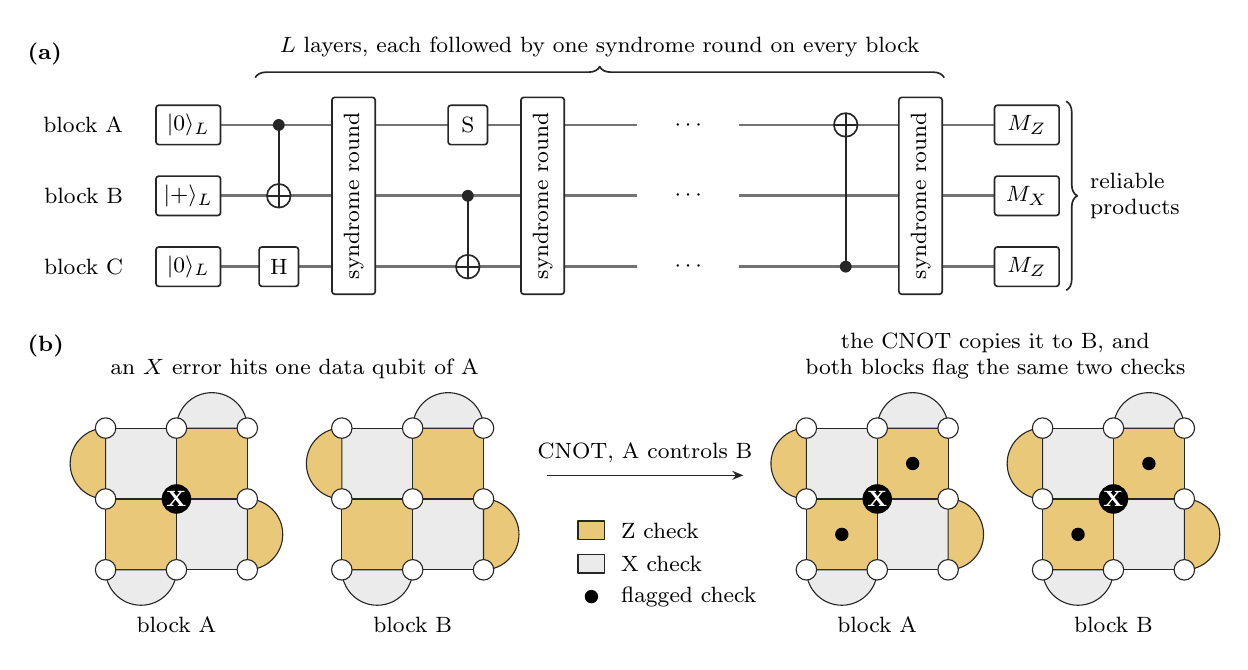
\begin{tikzpicture}[figbase,
  wire/.style={fheavy,draw=black!55},
  gate/.style={fbox,minimum height=0.5cm,minimum width=0.5cm,inner sep=1.5pt},
  dq/.style={circle,draw=fline,fill=white,fthin,minimum size=2.6mm,inner sep=0pt},
  err/.style={circle,draw=black,fill=black,fthin,minimum size=3.6mm,inner sep=0pt,text=white,font=\footnotesize\bfseries},
  flag/.style={circle,fill=black,minimum size=1.7mm,inner sep=0pt},
  chk/.style={draw=fline,fthin},
  panel/.style={anchor=north west,font=\footnotesize\bfseries,inner sep=0pt}]
% ---------- (a) the circuit ----------
\begin{scope}[shift={(0,4.6)}]
  \node[panel] at (0,2.85) {(a)};
  \foreach \y/\b in {1.8/A,0.9/B,0/C}{
    \node[anchor=east] at (1.35,\y) {block \b};
    \draw[wire] (2.05,\y)--(7.75,\y) (9.05,\y)--(12.7,\y);
    \node at (8.4,\y) {$\cdots$};
  }
  \foreach \y/\s in {1.8/0,0.9/+,0/0}{\node[gate,minimum width=0.82cm] at (2.05,\y) {$|\s\rangle_L$};}
  \foreach \y/\m in {1.8/Z,0.9/X,0/Z}{\node[gate,minimum width=0.82cm] at (12.7,\y) {$M_\m$};}
  % layer 1: CNOT A->B and H on C; layer 2: CNOT B->C and S on A; layer L: CNOT C->A with B idle
  \foreach \x/\c/\t in {3.2/1.8/0.9, 5.6/0.9/0, 10.4/0/1.8}{
    \draw[fmid] (\x,\c)--(\x,\t);
    \fill[fline] (\x,\c) circle (0.075);
    \draw[fmid,fill=white] (\x,\t) circle (0.15);
    \draw[fmid] (\x-0.15,\t)--(\x+0.15,\t) (\x,\t-0.15)--(\x,\t+0.15);
  }
  \node[gate] at (3.2,0) {H};
  \node[gate] at (5.6,1.8) {S};
  \foreach \x in {4.15,6.55,11.35}{\node[fbox,rotate=90,minimum width=2.5cm,minimum height=0.55cm,inner sep=1pt] at (\x,0.9) {syndrome round};}
  \draw[fmid,decorate,decoration={brace,amplitude=4pt}] (2.9,2.4)--(11.65,2.4)
    node[midway,above=4pt] {$L$ layers, each followed by one syndrome round on every block};
  \draw[fmid,decorate,decoration={brace,amplitude=4pt}] (13.2,2.1)--(13.2,-0.3)
    node[midway,right=5pt,align=left] {reliable\\products};
\end{scope}
% ---------- (b) the CNOT copies an X error ----------
\def\patch#1#2#3#4{% origin x, origin y, X error on the centre qubit (0/1), flagged checks (0/1)
  \begin{scope}[shift={(#1,#2)}]
    % weight-4 checks: Z where i+j is even, X where it is odd
    \foreach \i in {0,1}{\foreach \j in {0,1}{
      \pgfmathtruncatemacro{\pty}{mod(\i+\j,2)}
      \ifnum\pty=0 \filldraw[chk,fill=fzchk] (0.9*\i,0.9*\j) rectangle +(0.9,0.9);
      \else \filldraw[chk,fill=fxchk] (0.9*\i,0.9*\j) rectangle +(0.9,0.9);\fi
    }}
    % weight-2 boundary checks: X on top and bottom, Z on left and right
    \filldraw[chk,fill=fxchk] (0.9,1.8) arc[start angle=180,end angle=0,radius=0.45] -- cycle;
    \filldraw[chk,fill=fxchk] (0,0) arc[start angle=180,end angle=360,radius=0.45] -- cycle;
    \filldraw[chk,fill=fzchk] (0,1.8) arc[start angle=90,end angle=270,radius=0.45] -- cycle;
    \filldraw[chk,fill=fzchk] (1.8,0) arc[start angle=-90,end angle=90,radius=0.45] -- cycle;
    \ifnum#4=1 \node[flag] at (0.45,0.45) {}; \node[flag] at (1.35,1.35) {};\fi
    \foreach \i in {0,1,2}{\foreach \j in {0,1,2}{\node[dq] at (0.9*\i,0.9*\j) {};}}
    \ifnum#3=1 \node[err] at (0.9,0.9) {X};\fi
  \end{scope}}
\node[panel] at (0,3.75) {(b)};
\patch{1.0}{0.75}{1}{0}
\patch{4.0}{0.75}{0}{0}
\patch{9.9}{0.75}{1}{1}
\patch{12.9}{0.75}{1}{1}
\foreach \x/\b in {1.9/A,4.9/B,10.8/A,13.8/B}{\node[anchor=base] at (\x,-0.05) {block \b};}
\node[anchor=south] at (3.4,3.05) {an $X$ error hits one data qubit of A};
\node[anchor=south,align=center] at (12.3,3.05) {the CNOT copies it to B, and\\both blocks flag the same two checks};
\draw[flow] (6.6,1.95)--(9.1,1.95) node[midway,above=1pt] {CNOT, A controls B};
\begin{scope}[shift={(7.0,1.25)}]
  \foreach \y/\c/\t in {0/fzchk/Z check,-0.42/fxchk/X check}{
    \filldraw[chk,fill=\c] (0,\y-0.12) rectangle +(0.34,0.24);
    \node[anchor=west] at (0.42,\y) {\t};
  }
  \node[flag] at (0.17,-0.84) {};
  \node[anchor=west] at (0.42,-0.84) {flagged check};
\end{scope}
\end{tikzpicture}
 inside figure*.
\documentclass[multi=tikzpicture,border=4pt]{standalone}
\usepackage{tikz}
\usetikzlibrary{arrows.meta,decorations.pathreplacing,positioning,calc}
% Shared look of the four figures. Figs. 1 and 2 draw with these styles, and scripts/figures.py repeats the colours and
% line weights for Figs. 3 and 4. Colours: Paul Tol's high-contrast scheme (colour-blind safe, three distinct greys in
% greyscale), one meaning each in every figure:
%   fnet  #004488  the network                    fcomp #BB5566  the composition with Tesseract
%   black          baselines, errors and detection events of a shot
%   fzchk #E9C87A  Z checks (tint of #DDAA33)     fxchk #EBEBEB  X checks (lightness 82 and 93)
% Text 8 pt (\footnotesize, the caption is 9 pt). Lines 0.4 pt (fine detail), 0.6 pt (boxes, arrows, axes), 1.0 pt
% (wires, exchange, data lines). One arrow tip, one box (rounded 1 pt, its fill gives its role).
\definecolor{fnet}{HTML}{004488}
\definecolor{fcomp}{HTML}{BB5566}
\definecolor{fzchk}{HTML}{E9C87A}
\definecolor{fxchk}{HTML}{EBEBEB}
\colorlet{fnetbg}{fnet!10}
\colorlet{fcompbg}{fcomp!26}
\colorlet{fline}{black!85}
\tikzset{
  figbase/.style={x=1cm,y=1cm,font=\footnotesize,line width=0.6pt,draw=fline,line join=round,
    >={Stealth[length=4pt,width=3.2pt]}},
  fthin/.style={line width=0.4pt},
  fmid/.style={line width=0.6pt},
  fheavy/.style={line width=1pt},
  fbox/.style={draw=fline,line width=0.6pt,rounded corners=1pt,fill=white,inner sep=2.5pt,minimum height=0.6cm,
    align=center},
  flow/.style={->,draw=fline,line width=0.6pt},
}

\newcommand{\tess}{Tesseract}
\begin{document}
% Figure 1: a circuit on K = 3 blocks (a) and how a CNOT copies an X error between two blocks (b). Drawn at the width
% of the page (figure* environment, no scaling) in the shared figure style of figstyle.tex.
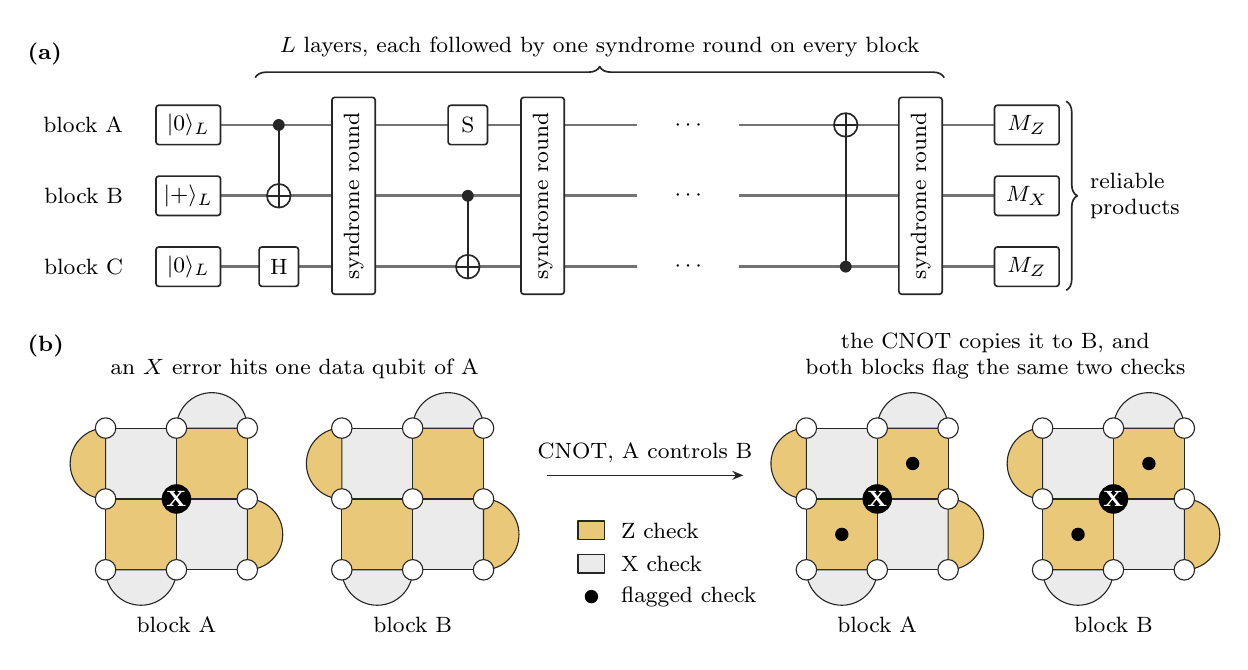
\begin{tikzpicture}[figbase,
  wire/.style={fheavy,draw=black!55},
  gate/.style={fbox,minimum height=0.5cm,minimum width=0.5cm,inner sep=1.5pt},
  dq/.style={circle,draw=fline,fill=white,fthin,minimum size=2.6mm,inner sep=0pt},
  err/.style={circle,draw=black,fill=black,fthin,minimum size=3.6mm,inner sep=0pt,text=white,font=\footnotesize\bfseries},
  flag/.style={circle,fill=black,minimum size=1.7mm,inner sep=0pt},
  chk/.style={draw=fline,fthin},
  panel/.style={anchor=north west,font=\footnotesize\bfseries,inner sep=0pt}]
% ---------- (a) the circuit ----------
\begin{scope}[shift={(0,4.6)}]
  \node[panel] at (0,2.85) {(a)};
  \foreach \y/\b in {1.8/A,0.9/B,0/C}{
    \node[anchor=east] at (1.35,\y) {block \b};
    \draw[wire] (2.05,\y)--(7.75,\y) (9.05,\y)--(12.7,\y);
    \node at (8.4,\y) {$\cdots$};
  }
  \foreach \y/\s in {1.8/0,0.9/+,0/0}{\node[gate,minimum width=0.82cm] at (2.05,\y) {$|\s\rangle_L$};}
  \foreach \y/\m in {1.8/Z,0.9/X,0/Z}{\node[gate,minimum width=0.82cm] at (12.7,\y) {$M_\m$};}
  % layer 1: CNOT A->B and H on C; layer 2: CNOT B->C and S on A; layer L: CNOT C->A with B idle
  \foreach \x/\c/\t in {3.2/1.8/0.9, 5.6/0.9/0, 10.4/0/1.8}{
    \draw[fmid] (\x,\c)--(\x,\t);
    \fill[fline] (\x,\c) circle (0.075);
    \draw[fmid,fill=white] (\x,\t) circle (0.15);
    \draw[fmid] (\x-0.15,\t)--(\x+0.15,\t) (\x,\t-0.15)--(\x,\t+0.15);
  }
  \node[gate] at (3.2,0) {H};
  \node[gate] at (5.6,1.8) {S};
  \foreach \x in {4.15,6.55,11.35}{\node[fbox,rotate=90,minimum width=2.5cm,minimum height=0.55cm,inner sep=1pt] at (\x,0.9) {syndrome round};}
  \draw[fmid,decorate,decoration={brace,amplitude=4pt}] (2.9,2.4)--(11.65,2.4)
    node[midway,above=4pt] {$L$ layers, each followed by one syndrome round on every block};
  \draw[fmid,decorate,decoration={brace,amplitude=4pt}] (13.2,2.1)--(13.2,-0.3)
    node[midway,right=5pt,align=left] {reliable\\products};
\end{scope}
% ---------- (b) the CNOT copies an X error ----------
\def\patch#1#2#3#4{% origin x, origin y, X error on the centre qubit (0/1), flagged checks (0/1)
  \begin{scope}[shift={(#1,#2)}]
    % weight-4 checks: Z where i+j is even, X where it is odd
    \foreach \i in {0,1}{\foreach \j in {0,1}{
      \pgfmathtruncatemacro{\pty}{mod(\i+\j,2)}
      \ifnum\pty=0 \filldraw[chk,fill=fzchk] (0.9*\i,0.9*\j) rectangle +(0.9,0.9);
      \else \filldraw[chk,fill=fxchk] (0.9*\i,0.9*\j) rectangle +(0.9,0.9);\fi
    }}
    % weight-2 boundary checks: X on top and bottom, Z on left and right
    \filldraw[chk,fill=fxchk] (0.9,1.8) arc[start angle=180,end angle=0,radius=0.45] -- cycle;
    \filldraw[chk,fill=fxchk] (0,0) arc[start angle=180,end angle=360,radius=0.45] -- cycle;
    \filldraw[chk,fill=fzchk] (0,1.8) arc[start angle=90,end angle=270,radius=0.45] -- cycle;
    \filldraw[chk,fill=fzchk] (1.8,0) arc[start angle=-90,end angle=90,radius=0.45] -- cycle;
    \ifnum#4=1 \node[flag] at (0.45,0.45) {}; \node[flag] at (1.35,1.35) {};\fi
    \foreach \i in {0,1,2}{\foreach \j in {0,1,2}{\node[dq] at (0.9*\i,0.9*\j) {};}}
    \ifnum#3=1 \node[err] at (0.9,0.9) {X};\fi
  \end{scope}}
\node[panel] at (0,3.75) {(b)};
\patch{1.0}{0.75}{1}{0}
\patch{4.0}{0.75}{0}{0}
\patch{9.9}{0.75}{1}{1}
\patch{12.9}{0.75}{1}{1}
\foreach \x/\b in {1.9/A,4.9/B,10.8/A,13.8/B}{\node[anchor=base] at (\x,-0.05) {block \b};}
\node[anchor=south] at (3.4,3.05) {an $X$ error hits one data qubit of A};
\node[anchor=south,align=center] at (12.3,3.05) {the CNOT copies it to B, and\\both blocks flag the same two checks};
\draw[flow] (6.6,1.95)--(9.1,1.95) node[midway,above=1pt] {CNOT, A controls B};
\begin{scope}[shift={(7.0,1.25)}]
  \foreach \y/\c/\t in {0/fzchk/Z check,-0.42/fxchk/X check}{
    \filldraw[chk,fill=\c] (0,\y-0.12) rectangle +(0.34,0.24);
    \node[anchor=west] at (0.42,\y) {\t};
  }
  \node[flag] at (0.17,-0.84) {};
  \node[anchor=west] at (0.42,-0.84) {flagged check};
\end{scope}
\end{tikzpicture}

% Figure 2: the network and the composition, drawn at the width of the page (figure* environment, no scaling) in the
% shared figure style of figstyle.tex. Blue boxes hold the learned weights, white boxes compute exactly, and the
% rose box is Tesseract, as in Figs. 3 and 4.
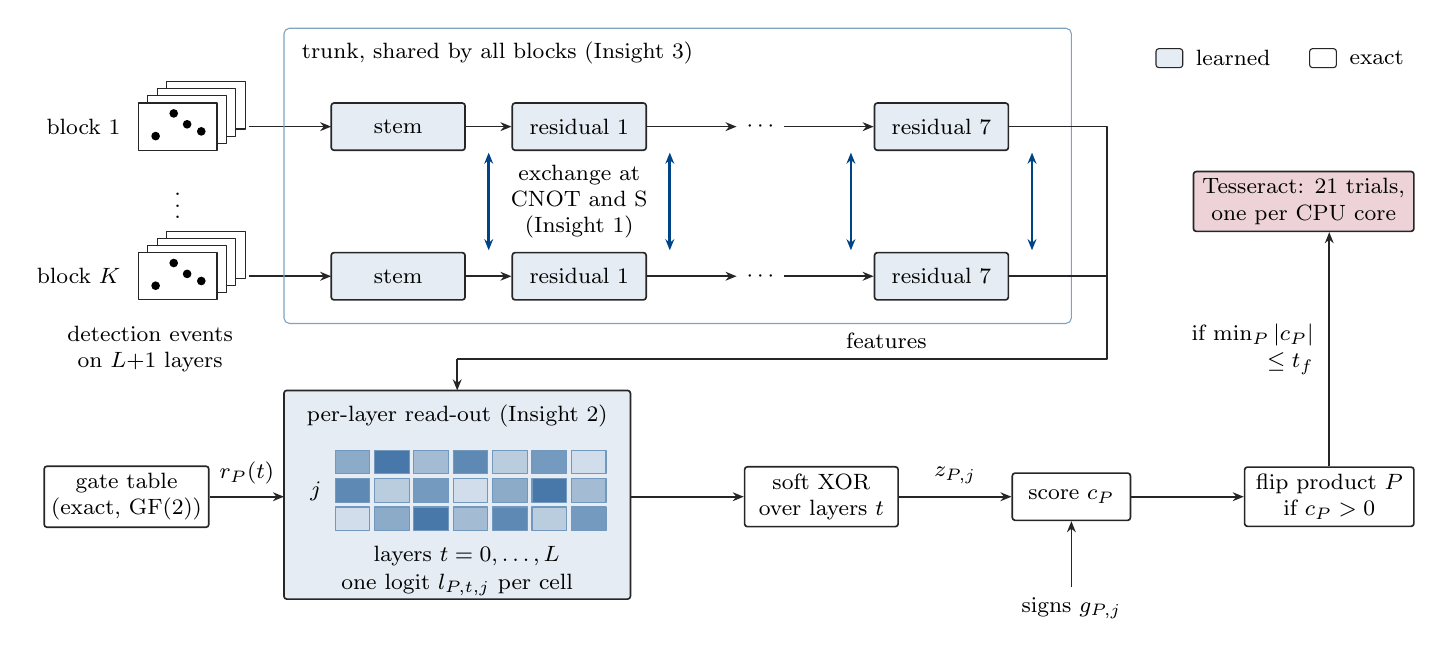
\begin{tikzpicture}[figbase,
  card/.style={draw=fline,fill=white,fthin},
  ev/.style={circle,fill=black,inner sep=0pt,minimum size=1.1mm},
  learned/.style={fbox,fill=fnetbg},
  exch/.style={<->,fheavy,draw=fnet},
  key/.style={draw=fline,fthin,rounded corners=1pt}]
\def\ya{6.3}\def\yk{4.4}
% ---------- row 1: detection events of every block and the trunk ----------
\foreach \y in {\ya,\yk}{
  \foreach \k in {3,2,1,0}{\draw[card] (0.9+0.12*\k,\y-0.3+0.09*\k) rectangle +(1.0,0.6);}
  \foreach \px/\py in {0.22/0.2,0.62/0.45,0.45/0.68,0.8/0.3}{\node[ev] at (0.9+\px,\y-0.3+\py*0.6+0.06) {};}
  \draw[flow] (2.3,\y)--(3.35,\y);
}
\node[anchor=east] at (0.8,\ya) {block 1};
\node[anchor=east] at (0.8,\yk) {block $K$};
\node at (1.4,5.4) {$\vdots$};
\node[anchor=north,align=center] at (1.05,3.9) {detection events\\on $L{+}1$ layers};
\draw[draw=fnet!50,fthin,rounded corners=2pt] (2.75,3.8) rectangle (12.75,7.55);
\node[anchor=north west] at (2.85,7.5) {trunk, shared by all blocks (Insight 3)};
\foreach \y/\id in {\ya/a,\yk/b}{
  \node[learned,minimum width=1.7cm] (s\id) at (4.2,\y) {stem};
  \node[learned,minimum width=1.7cm] (r1\id) at (6.5,\y) {residual 1};
  \node (r2\id) at (8.8,\y) {$\cdots$};
  \node[learned,minimum width=1.7cm] (r7\id) at (11.1,\y) {residual 7};
  \draw[flow] (s\id)--(r1\id);
  \draw[flow] (r1\id)--(r2\id);
  \draw[flow] (r2\id)--(r7\id);
}
\foreach \x in {5.35,7.65,9.95,12.25}{\draw[exch] (\x,\ya-0.33)--(\x,\yk+0.33);}
\node[align=center] at (6.5,5.35) {exchange at\\CNOT and S\\(Insight 1)};
% ---------- trunk output to the read-out ----------
\draw[fmid] (r7a.east)--(13.2,\ya)--(13.2,3.35)--(4.95,3.35);
\draw[fmid] (r7b.east)--(13.2,\yk);
\draw[flow] (4.95,3.35)--(4.95,2.95);
\node[anchor=south] at (10.4,3.35) {features};
% ---------- row 2: gate table, per-layer read-out, soft XOR, score ----------
\node[fbox,minimum width=2.0cm] (tab) at (0.75,1.6) {gate table\\(exact, GF(2))};
\draw[learned] (2.75,0.3) rectangle (7.15,2.95);
\node[anchor=north] at (4.95,2.9) {per-layer read-out (Insight 2)};
\foreach \t in {0,...,6}{\foreach \j in {0,1,2}{
  \pgfmathsetmacro{\sh}{18+9*mod(\t*3+\j*5,7)}
  \filldraw[fthin,draw=fnet!55,fill=fnet!\sh] (3.4+0.5*\t,1.17+0.36*\j) rectangle +(0.44,0.3);
}}
\node[anchor=east] at (3.35,1.67) {$j$};
\node[anchor=north] at (5.07,1.1) {layers $t=0,\dots,L$};
\node[anchor=north] at (4.95,0.75) {one logit $l_{P,t,j}$ per cell};
\draw[flow] (tab.east)--(2.75,1.6) node[midway,above=1pt] {$r_P(t)$};
\node[fbox,minimum width=1.95cm] (xor) at (9.575,1.6) {soft XOR\\over layers $t$};
\draw[flow] (7.15,1.6)--(xor.west);
\node[fbox,minimum width=1.5cm] (sc) at (12.75,1.6) {score $c_P$};
\draw[flow] (xor.east)--(sc.west) node[midway,above=1pt] {$z_{P,j}$};
\draw[flow] (12.75,0.45)--(sc.south);
\node[anchor=north] at (12.75,0.45) {signs $g_{P,j}$};
\node[fbox,minimum width=2.15cm] (out) at (16.025,1.6) {flip product $P$\\if $c_P>0$};
\draw[flow] (sc.east)--(out.west);
% ---------- composition: unsure shots go to Tesseract ----------
\node[fbox,fill=fcompbg,minimum width=2.8cm] (tess) at (15.7,5.35) {\tess: 21 trials,\\one per CPU core};
\draw[flow] (out.north)--(out.north|-tess.south) node[midway,left=2pt,align=right] {if $\min_P|c_P|$\\${}\le t_f$};
% ---------- key ----------
\node[anchor=east] (k2) at (17.1,7.17) {exact};
\draw[key,fill=white] ($(k2.west)+(-0.38,-0.12)$) rectangle +(0.34,0.24);
\node[anchor=east] (k1) at ($(k2.west)+(-0.75,0)$) {learned};
\draw[key,fill=fnetbg] ($(k1.west)+(-0.38,-0.12)$) rectangle +(0.34,0.24);
\end{tikzpicture}

\end{document}
